\section{Singapour, ville? pays?}

Date: 09/05/2008

\begin{multicols}{2}

Une fois n'est pas coutume, c'est deux articles que je vous écris aujourd'hui, je vous propose donc de retourner voir dans la rubrique Indonésie, l'article sur Bornéo.

Nous voici rendus à Singapour.

La première vue de cette ville, c'est le détroit de Malacca que nous passons en bateau, ce détroit est très impressionnant de par le nombre de cargos et portes conteners qui y sont arrétés, sans doute en attente de disponibilité d'un quai sur le port, pour pouvoir décharger. En effet Singapour est le plus gros port de commerce du monde, je croyais qu'il s'agissait de Rotterdam mais on m'a affirmé ici que c'etait Singapour, et à voir le traffic qu'il s'y passe, je veux bien le croire.

%<div><object width="640" height="505"><param name="movie" value="http://www.dailymotion.com/swf/x5d3be&v3=1&related=1"></param><param name="allowFullScreen" value="true"></param><param name="allowScriptAccess" value="always"></param><embed src="http://www.dailymotion.com/swf/x5d3be&v3=1&related=1" type="application/x-shockwave-flash" width="640" height="505" allowFullScreen="true" allowScriptAccess="always"></embed></object></div>

Voici une toute petite partie du port, nous l'avons longé durant 3 heure, c'est dire si il est long !!!

\hspace*{-0.65cm}
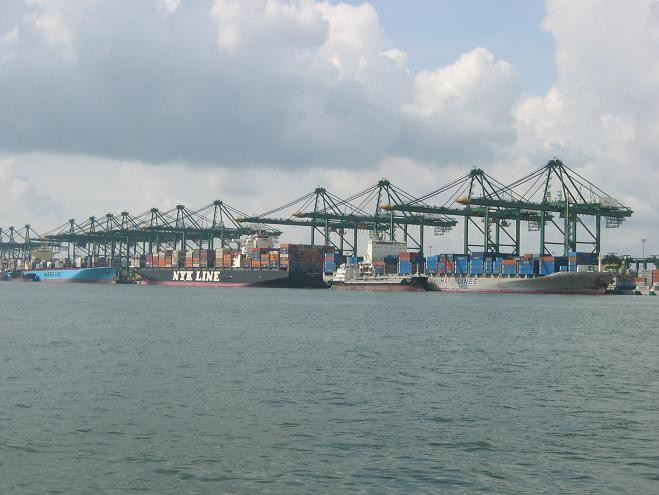
\includegraphics[width=4.8cm]{articles/Singapour-ville-pays/1210333644359c.jpg}
Port de Singapour.

Que vous dire sur Singapour ???

Pour être clair, nous avons étés déçus par cette ville, trop clean, enclave de business au milieu de l'Asie. Je pourrais vous décrire avec de plus amples détails cette ville mais je vais préférer une image : Prenez la complexité d'une ville comme Paris, ajoutez y la propreté de Geneve (les amendes hors de prix pour le simple fait de jeter un papier faisant partie de la propreté) et rajoutez à cela un boom économique, des constructions nouvelles, comme dans un pays de pétrole, Dubaï, aux Emirats Arabes. Vous obtenez Singapour. Certe tout le monde parle anglais, on paie en dollars, tout est propre... mais pour moi il manque quelque chose !!!

Le tout vous donne une impression d'étouffer, cette ville est sympa à visiter mais pour rien au monde je ne viendrai y habiter.

Enclave parmis cela : Chinatown, le quartier chinois, où je retrouve le bordel que j'aime, ça grouille de partout, ça négocie, ça arnaque, il y a des boutiques de partout, sur on ne sait combien d'étages... Et nos cher geek trouveraient leur bonheur à Sim Lim Square, gros building de 7 étages entièrement remplis de boutiques d'informatiques, nous en avons profité pour faire réparer l'ordinateur portable qui nous avait laché juste après Bornéo. Et comme il etait vieux, Patrick se disant qu'il allait bientôt re-lâcher, il en a acheté un nouveau, résultat nous avons deux ordinateurs portables à bord... Et moi qui voulais faire un break !?!??!!?

Je vous laisse sur une photo de la marina où nous sommes restés durant notre séjour à Singapour.

\hspace*{-0.65cm}
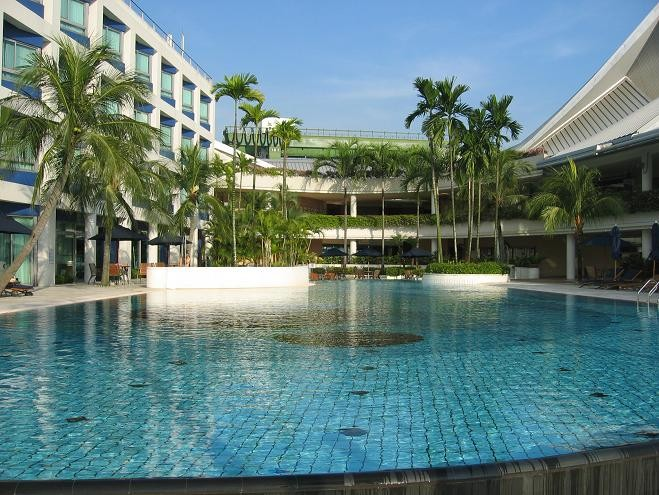
\includegraphics[width=4.8cm]{articles/Singapour-ville-pays/1210345462qOEk.jpg}
Piscine de la marina.

A savoir : Le propriétaire d'un bateau ici est considéré comme étant obligatoirement riche, il n'existe donc pas de marina bon marché, le luxe est obligatoire (non je n'éxagere pas). Cela dit pour un "western" cela reste à la portée des bourses les plus légères, mais se voir proposer tout ce luxe est déconcertant à la fin, ça contraste avec nos journées en mer à prendre des douches à l'eau de mer, et uniquement se rincer à l'eau douce.

\end{multicols}

\bigskip
\textbf{\textsc{Commentaires}}

\medskip
Titou a écrit le 09 mai 2008 :
\begin{displayquote}
Ra ti Dud !! ne te plaint pas d'être dans un cadre idyllique malgré un luxe trop présent à ton goût ! Continue de profiter et de nous faire partager tes aventures ! Ça m'a fait super plaisir de t'avoir en direct et j'espère qu'on aura l'occaz de se recroiser sur le net d'ici peu ! D'ici la enjoy and take care !
Biz ma poule
\end{displayquote}

\medskip
Mamam titou a écrit le 15 mai 2008 :
\begin{displayquote}
c'est toujours agréable de pouvoir suivre ton périple et la photo de la marina m'a laissé réveuse ... cadre idyllique - continues d'en profiter jusqu'au bout et comme le dit si bien titou : enjoy and take care.
\end{displayquote}

\medskip
Gege a écrit le 19 mai 2008 :
\begin{displayquote}
Salut dud,
pour le port de Rotterdam, je crois que c'est seulement le premier port européen (après vérification, c'est ça. Singapour à pris le dessus en 2003 et Shangai en 2005)
Sinon, je comprend totalement ton désintéressement pour ce genre de villes...
C'est pas tout à fait la vie "réelle"
\end{displayquote}

\vfill

